\documentclass[../../General.tex]{subfiles}
\begin{document}


\section{Diagrama de operaciones}

    Para diferenciar las responsabilidades y los canales de interacción de cada actor identificado en el análisis de stakeholders, la descripción se divide en dos diagramas independientes: el Usuario Principal (Técnico de O\&M en campo) y el Usuario Directo (Gestor de Activos y Auditor O\&M remoto).En ambos esquemas, se utiliza la simbología estandarizada donde los símbolos circulares representan procedimientos o comandos ejecutados por el usuario, mientras que los rombos y rectángulos representan subrutinas, decisiones lógicas y respuestas automáticas ejecutadas por el robot.

    \subsection{Flujo de operación del Usuario Principal}

    El flujo de trabajo, observado en la Figura \ref{fig:DiagramaOperaciones1}, en campo consta de cuatro fases secuenciales y paralelas: El procedimiento inicia en el taller o punto de alistamiento de la planta fotovoltaica. El técnico realiza la inspección óptica del domo del piranómetro Clase A y de la lente del módulo de cámara CMOS. A continuación, inserta en la ranura externa la tarjeta de memoria MicroSD con el archivo de coordenadas de los pasillos, y acciona el interruptor principal. La SBC arranca el sistema operativo, ejecuta el autodiagnóstico de buses y despliega la lectura de estado en la pantalla LCD local. A continuación, el técnico traslada el UGV a la cabecera del pasillo entre seguidores solares, selecciona la ruta navegando en la pantalla LCD local y presiona el botón de confirmación en la interfaz LCD para autorizar el inicio del ciclo autónomo. En la siguiente fase, la SBC ejecuta tres hilos concurrentes en tiempo real:

    \begin{itemize}
        \item \textbf{Inspección Climática:} El servomotor del elevador de tijera despliega la plataforma a una altura $h \ge 1300 \text{ mm}$ del suelo, mientras el goniómetro de 1 eje  alinea el piranómetro Clase A con el ángulo Tilt de los paneles. La tracción diferencial avanza siguiendo el algoritmo Pure Pursuit.
        \item \textbf{Percepción y Evasión Local:} La cámara CMOS frontal monitorea un semicírculo de $1 \text{ m}$. Si se detecta un obstáculo (maleza, rocas o herramientas), la SBC calcula una desviación local, esquiva el obstáculo, se reincorpora al pasillo fotovoltaico y continúa la misión de medición sin interrumpir el recorrido.
        \item \textbf{Supervisión Energética:} El contador de Culombios del BMS monitorea la descarga de las celdas. Únicamente si el nivel cae por debajo del $15\%$, el sistema aborta la inspección, repliega los mecanismos articulados a posición de transporte y ejecuta la subrutina de Retorno Automático navegando de vuelta al punto inicial del pasillo.
    \end{itemize}


    \begin{figure}[H]
        \captionsetup{justification=raggedright, singlelinecheck=false, labelsep=none}
        \caption[Flujo de operación del Usuario Principal.]{} 
        \textit{Flujo de operación del Usuario Principal.} \par\medskip
        
        \centering
        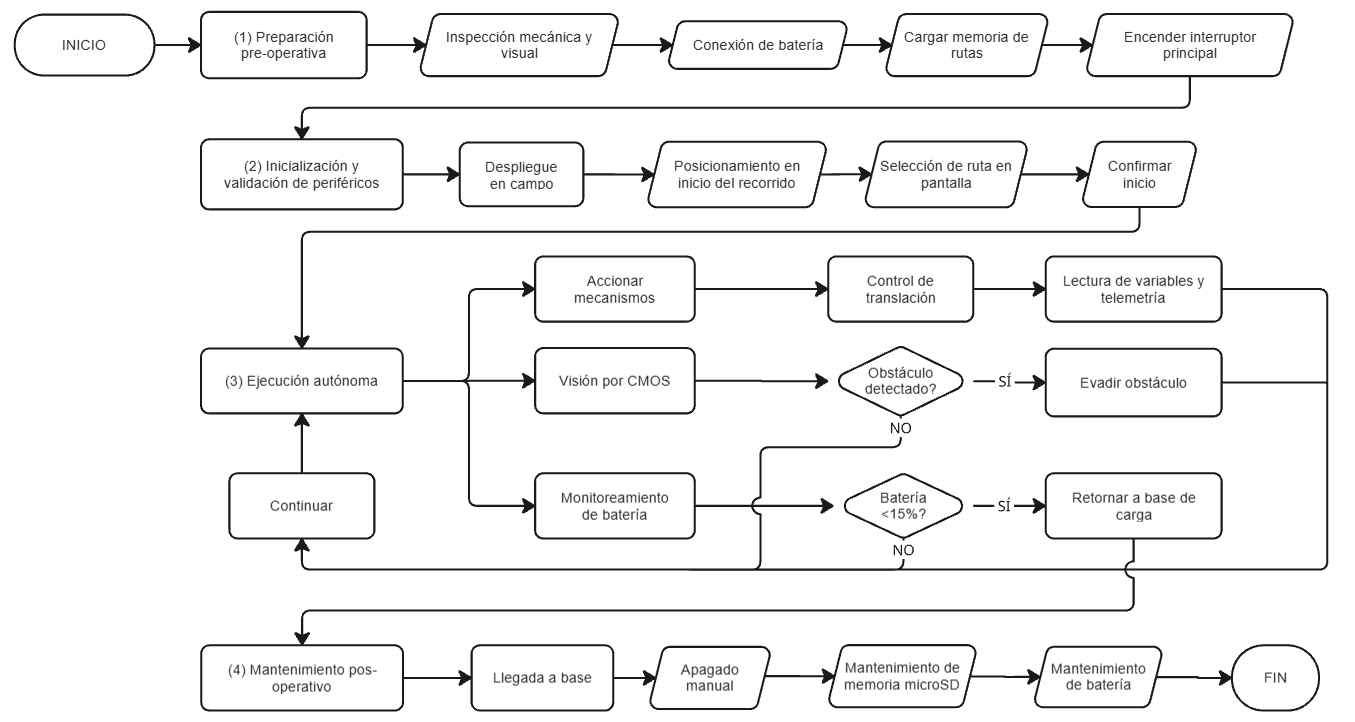
\includegraphics[width=0.8\textwidth]{Recursos/Imagenes/ImagenesDisenoProgramacion/FlujoOperaciones1.png} \par\medskip
        
        \raggedright
        \footnotesize \textit{Nota.} Elaboración propia.
        \label{fig:DiagramaOperaciones1}
    \end{figure}


    Finalmente, al llegar a la cabecera inicial (por ruta completada o retorno por batería baja), el robot notifica el mensaje en la pantalla LCD local. El técnico apaga el equipo desde el seccionador, extrae la tarjeta MicroSD para el respaldo no volátil de la base de datos climática, limpia el piranómetro y conecta la batería al cargador comercial.


    \subsection{Flujo de operación del Usuario Directo}

    El siguiente flujo, observado en la Figura \ref{fig:DiagramaOperaciones2}, describe la operación del auditor o gestor de telemetría, el cual accede al Dashboard web del centro de control mediante credenciales encriptadas. La plataforma establece comunicación inalámbrica con el Gateway central del parque solar, verificando los indicadores de calidad de radiofrecuencia y desplegando la cartografía vectorial de los pasillos; a continuación, el usuario configura la frecuencia de transmisión telemétrica y emite la instrucción inalámbrica de inicio, el paquete se transmite por LoRa al robot.Durante el desplazamiento del UGV en el pasillo, el servidor decodifica continuamente las tramas de carga útil enviadas por el robot. Si se detecta una condición crítica, el Dashboard resalta la alerta en color rojo en el mapa GPS exacto, permitiendo al gestor pulsar el botón de Parada Remota de Emergencia vía LoRa. Al concluir el recorrido, el robot emite la trama de cierre de ruta. El auditor ejecuta el algoritmo de integración climática para calcular el PR definitivo de la planta corregido por temperatura, cuantifica las pérdidas asociadas al soiling y exporta el informe técnico-económico de auditoría en formato PDF/Excel para sustentar las garantías de generación ante los inversionistas u operadores de red.


    \begin{figure}[H]
        \captionsetup{justification=raggedright, singlelinecheck=false, labelsep=none}
        \caption[Flujo de operación de.]{}
        \textit{Flujo de operación de.} \par\medskip
        
        \centering
        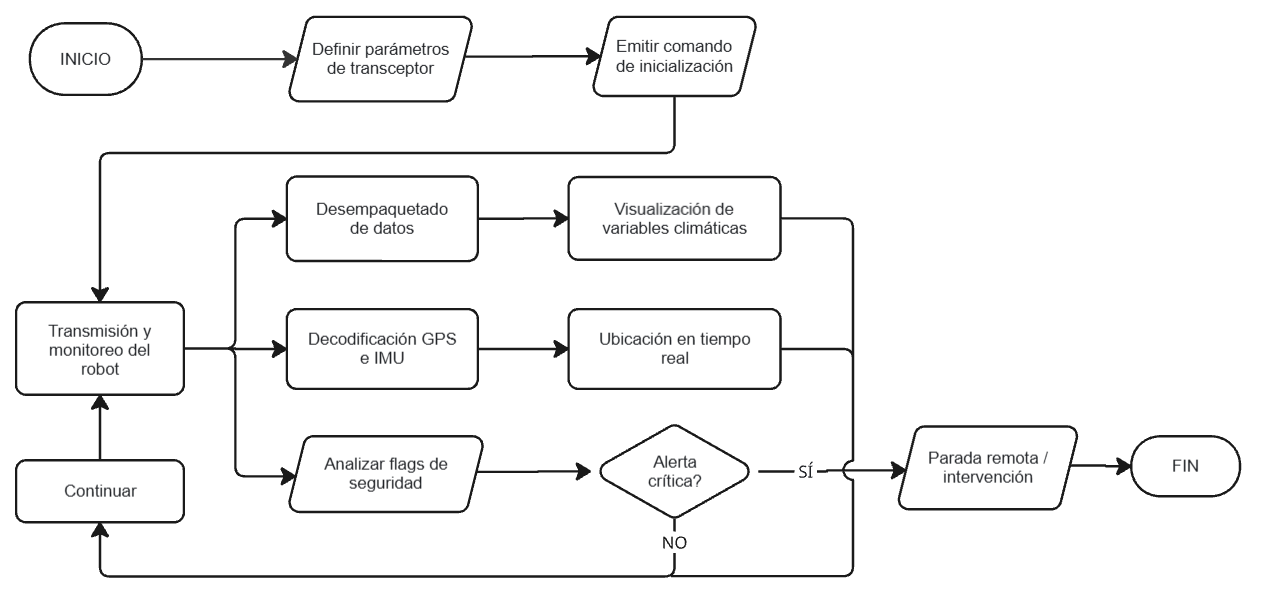
\includegraphics[width=0.8\textwidth]{Recursos/Imagenes/ImagenesDisenoProgramacion/FlujoOperaciones2.png} \par\medskip
        
        \raggedright
        \footnotesize \textit{Nota.} Elaboración propia.
        \label{fig:DiagramaOperaciones2}
    \end{figure}

\end{document}